\documentclass[a4paper, 11pt]{article}
\usepackage{comment} % enables the use of multi-line comments (\ifx \fi) 
\usepackage{fullpage} % changes the margin
\usepackage{graphicx}

\begin{document}

\begin{center}
\textbf{\Large{Network Auto Tester and Evaluator}}\\
\textbf{NATE}
\end{center}

\noindent
\large\textbf{Documentation for V.3.0} \hfill \textbf{by: Andrey G.} \\
\normalsize  \hfill \\
\hfill Generate on: \today 

\section{Network Training and Testing}
Network Auto Tester and Evaluator (NATE) is a framework for automatic training neural networks and evaluating their performance efficiency. The framework allows to design a set of neural network based experiments that will be executed consequently in an automatic manner. Each task allows to specify a neural network architecture, training parameters, datasets, and data augmentation methods - thus allowing to analyze which particular combination of parameters yield the best result in a specific research study. 

The main advantage of the NATE framework is that it frees the user from mundane work of manually launching networks permitting to focus on more important stage of investigation such as network design and result analysis. The standartized procedure of saving intermideate logs, network efficiency measurements and network predictions on a test set also aids with analysis of the results allowing to redo the previous experiments with ease.  

\section{Quick Launch}

\subsection{Build Datasets}
Common dataset loaders implemented in the PyTorch framework operate by scanning the folder structure 

\subsection{Design Experiments and Create a Task File}
To carry automatic experimentation with different networks and parameters the user has to write the task file in the JSON format. Below there is an example of such file that contains 

\begin{verbatim}
{
  "tasklist":
  [
    {
      "tasktype": "class",
      "taskstage": "s2e",
      "taskcheckpoint": "",

      "database": "D:/ANDREY/DevXray/database/db-handai-imgs/",
      "dataset_train": "D:/ANDREY/DevXray/in_datasets/handai-03/s8510-t1/cls-s8510-t1-2016-test.txt",
      "dataset_validate": "D:/ANDREY/DevXray/in_datasets/handai-03/s8510-t1/cls-s8510-t1-2016-test.txt",
      "dataset_test": "D:/ANDREY/DevXray/in_datasets/handai-03/s8510-t1/cls-s8510-t1-2016-test.txt",

      "output_log": "D:/ANDREY/DevXray/out_mlog/handai-log/",
      "output_model": "D:/ANDREY/DevXray/out_mtar/handai-model/",
      "output_accuracy": "D:/ANDREY/DevXray/out_macc/handai-output/",

      "network": "densenet121",
      "network_istrained": true,
      "network_classcount": 1,
      "activation": "sigmoid",

      "trnsfrm_train": ["resize", "rndcrop"],
      "trnsfrm_train_param": [256, 224],
      "trnsfrm_validate": ["resize", "rndcrop"],
      "trnsfrm_validate_param": [256, 224],
      "trnsfrm_test": ["resize", "10Crop"],
      "trnsfrm_test_param": [256, 224],

      "loss": "WBCE",
      "epoch": 10,
      "lrate": 0.001,
      "batch": 32
    }
  ]
}
\end{verbatim}

This experiment task will carry start-to-end procedure of training and evaluating a network for solving a binary classification problem. The architecture of the network is DenseNet121 and the initial weights will be assigned from a pre-trained network (ImageNet, torchvision). The loss function used during training procedure is going to be weighted binary cross entropy, learning rate 0.001. The training will be done for 10 epochs with batch size of 32.

To create a new task the user should create a new text file with the formatting described below \footnote{The task file is a JSON file and follows the rules of this format.}.
Each individual task should be specified in the array \texttt{tasklist} surrounded by brackets \{ and \}.

\begin{itemize}
    \item \textbf{tasktype} - defines a type of task that will be carried out. This parameter can have the following string\texttt{Strings in JSON are surrounded by \"!} values: \textbf{class} - for classification task, 
    \textbf{img2img} - for image to image learning (autoencoder), \textbf{seg} - for segmentation task.
    
    \item \textbf{taskstage} - defines what stages of training and testing should be carried out. This parameter can have the following string values: \textbf{train} - for executing only training, \textbf{test} - for executing only testing, \textbf{resume} - for resuming the terminated start-to-end task, \textbf{s2e} - start-to-end task that includes training and testing stages
    
    \item \textbf{taskcheckpoint} - path to the trained model file that can be used for resuming the start-to-end procedure or conducting testing of the trained model. This parameter can be omitted for \textbf{train} and \textbf{s2e} task stages.
    
    \item \textbf{database} - path to the root directory for the image database. Image paths that are written in datasets should be relative to this path.
    
    \item \textbf{dataset\_train} - path to the training dataset file. This setup parameter can be omitted for \textbf{test} task stage.
    
    \item \textbf{dataset\_validate} - path to the validation dataset file. This setup parameter can be omitted for \textbf{test} task stage.
    
    \item \textbf{dataset\_test} - path to the test dataset file. This setup parameter can be omitted for \textbf{train} task stage.
    
    \item \textbf{output\_log} - path to a directory where a log file will be saved.
    
    \item \textbf{output\_model} - path to a directory where a trained network model will be saved.
    
    \item \textbf{output\_accuracy} - path to a directory where the evaluation metrics and results of testing will be saved.
    
    \item \textbf{network} - network architecture. The list of the supported architectures is the following:
    alexnet, convnet12, densenet121, densenet169, densenet201, inception, resnet50, resnet101, vggn16, hrdensenet121, hrdensenet169, scalenet3, fcdensenet103, fcdensenet50 \footnote{See section \ref{nnarch}}
    
    \item \textbf{network\_istrained} - a boolean flag. If set to \textbf{true} then a pre-trained network model is used (for torchvision networks). 
    
    \item \textbf{network\_classcount} - number of output classes if the task is to train a network for a classification or segmentation problems. Should be set up to 3 for image-to-image conversion tasks.
    
    \item \textbf{activation} - type of activation function. Supported only \textbf{sigmoid} and \textbf{softmax} and only for torchvision networks. 
    
    \item \textbf{trnsfrm\_train, trnsfrm\_validate, trnsfrm\_test} - image transformation sequence for the training, validation and test sets. Should be defined as an array and contain one or more (V3.0) transformations: \textbf{resize} - resize and image; \textbf{rndcrop} - random crop; \textbf{ccrop} - center crop; \textbf{10crop} - 10 crop\footnote{10 crop is supported only for testing!}
    
    \item \textbf{trnsfrm\_train\_param, trnsfrm\_validate\_param, trnsfrm\_test\_param} - parameters of the transformation. Should be defined as an array of similar size as the transformations array. The parameters should be specified according to the PyTorch transformation documentation.
	
	\item \textbf{trnsfrm\_seg\_end} - transformation sequence over the labeled maps for the segmentation task
	
	\item \textbf {trnsfrm\_seg\_end\_param} - transfromation sequence parameters for the labeled maps in case of the segmentation task
    
\end{itemize}



\section{Supported Network Architectures}
\label{nnarch}
The following architectures are supported in the NATE framework (V3.0 - Jan 2019).

\begin{itemize}
    \item AlexNet - torchvision implementation of the AlexNet architecture. Input image resolution is 224x224x3, output - N-dimensional vector.
    \item ConvNet12 - a shallow network of 12 convolutions and 6 pooling layers. Input image resolution is 224x224x3, output - N-dimensional vector.
    \item DenseNet121 - torchvision implementation of the DenseNet121 architecture. Input image resolution is 224x224x3, output - N-dimensional vector.
    \item DenseNet169 - torchvision implementation of the DenseNet169 architecture. Input image resolution is 224x224x3, output - N-dimensional vector.
    \item DenseNet201 - torchvision implementation of the DenseNet169 architecture. Input image resolution is 224x224x3, output - N-dimensional vector.
    \item Inception - torchvision implementation of the Inception architecture. Input image resolution is 224x224x3, output - N-dimensional vector.
    \item ResNet50 - torchvision implementation of the RenseNet50 architecture. Input image resolution is 224x224x3, output - N-dimensional vector.
    \item ResNet101 - torchvision implementation of the RenseNet101 architecture. Input image resolution is 224x224x3, output - N-dimensional vector.
    \item VGGN16 - torchvision implementation of the RenseNet101 architecture. Input image resolution is 224x224x3, output - N-dimensional vector.
    \item HRDenseNet121 - a DenseNet121 network which allows to supply 3-channel images of any resolution, output is an N-dimensional vector. 
    \item HRDenseNet169 - a DenseNet169 network which allows to supply 3-channel images of any resolution, output is an N-dimensional vector. 
    \item ScaleNet3 - a shallow architecture which contcatenates feature maps on different scales. Input image resolution is 227x227x3, output is an N-dimensional vector.
    \item FcDenseNet103 - DenseNet Teramisu (FC-DenseNet) with 103 layers. This network can be used for autoencoder tasks or segmentation. Any sensible resolution is supported for the input, but the input should have 3 channels. The output is the same resolution as the input, with N channels.
    \item FcDenseNet50 - DenseNet Teramisu (FC-DenseNet) with 50 layers. This network can be used for autoencoder tasks or segmentation. Any sensible resolution is supported for the input, but the input should have 3 channels. The output is the same resolution as the input, with N channels.

\end{itemize}

\begin{figure}
    \centering
    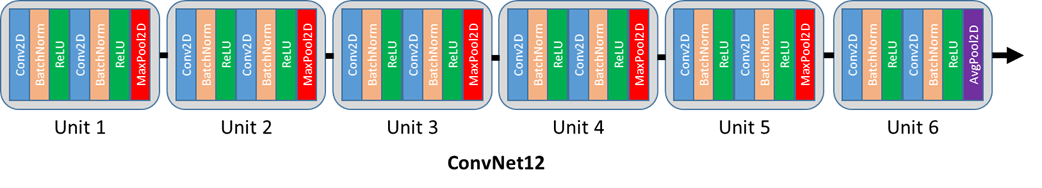
\includegraphics[width=0.8\textwidth]{img/convnet12.png}
    \caption{Architectuer of the ConvNet12 network}
    \label{convnet12}
\end{figure}

\section{Internal Architecture}
This section contains description of the internal architecture of the NATE framework and several tips on implementing new functionaslity.

%--------------------------------------------- WORKFLOW ---------------------------------------------
\subsection{Workflow}
The execution of the set of tasks specified in a JSON file is split into several stages. First the JSON is parsed and for each task a separated object that holds textural description of the task - \textbf{TaskSettings} - is created\footnote{Preliminary correctness checks are also done during JSON parsing}. 
These objects are gathered together in a list \textbf{TaskSettingsCollection}. Then the script enters the main procedural loop. It picks one task from the list of tasks and generates an execution environment checking the correctness of provided data \textbf{TaskEnvironment}. At the generation stage the network model, data loaders are created and file system environment variables are instantiated. The generation step is followed by execution stage where NATE carries out training and testing procedures. In the following sections detailed description of classes and modules is given.
\begin{figure}
    \centering
    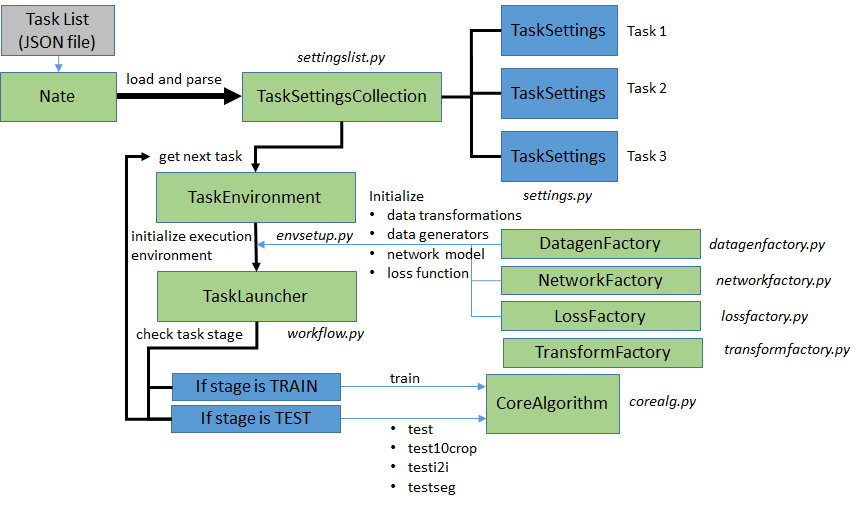
\includegraphics[width=0.8\textwidth]{img/schemenate1.png} 
    \caption{Workflow of the NATE training and testing procedure. At the first step the input JSON file is loaded with the class TaskSettingsCollection that creates a list of tasks consisting of objects TaskSettings. Next the necessary execution environment is initialized by generating necessary model, loss, data generators and other necessary objects using a number of factory classes. The execution is than handled to TaskLauncher class, that prepares specifies the environment for each stage of the task: training or testing. The immediated iteration through epochs and testing procedures are carried out then by CoreAlgorithm class.}
    \label{fig:my_label}
\end{figure}

%--------------------------------------------- MODULES ---------------------------------------------
\subsection{Modules}
The NATE framework is split into following separated modules
\begin{itemize}
    \item \textbf{datagen} (nate/datagen) - data generators and a factory for generating specific data generators
    \item \textbf{loss} (nate/loss) - a collection of custom loss functions and a factory class that returns a specific instance of a loss function by its name
    \item \textbf{network} (nate/network) - a collection of network classes and a factory for generating a particular network by specifying its name and additional parameters
    \item \textbf{score} (nate/score) - methods for evaluating the efficiency of the trained network (AUROC, F-score, Precision Recall etc)
    \item \textbf{settings} (nate/settings) - classes that describe parameters of an individual and multiple tasks
    \item \textbf{transform} (nate/transform) - a factory for initializing transfromations for data augmentations
\end{itemize}

\subsection{Module: network}
Module network\footnote{nate/network} contains python files that contains classes describing neural network architectures and contains an implementation of the network factory class \textbf{NetworkFactory}\footnote{See file netfactory.py}



\end{document}
